\section{Durchführung und Aufbau}
\label{sec:Durchführung}

Der Heizstrom der Kathode liegt in einem Bereich von ca. 2-3 A.
Für die Messung der Kennlinien wird folgende Schaltung verwendet.

\begin{figure}[H]
  \centering
  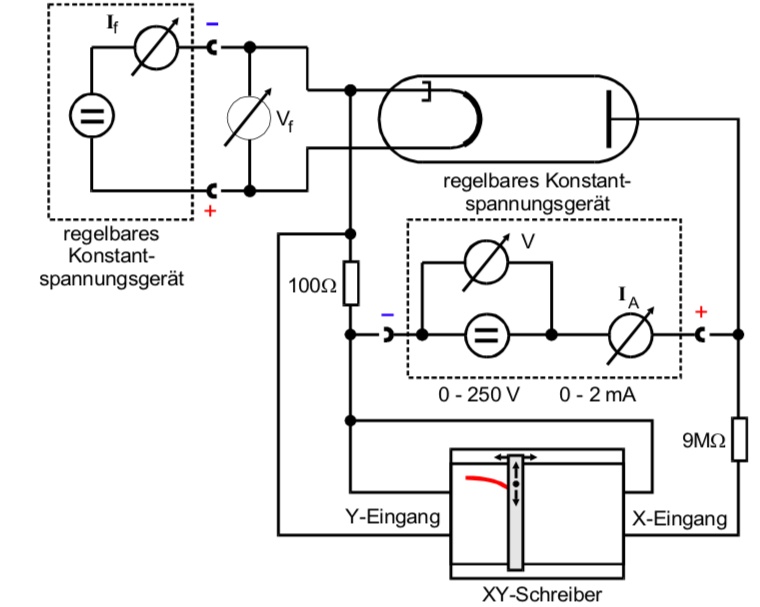
\includegraphics[width=0.8\textwidth]{content/7.png}
  \caption{Schaltung zur Aufnahme von Diodenkennlinien \cite{sample}}
  \label{fig:7}
\end{figure}

Ein Heizstrom und eine Heizspannung, beide ablesbar, werden in der Schaltung angestellt. Ein Konstantspannungsgerät
kann nun auch eine Spannung an die Diode anlegen. Der daraus resultierende Diodenstrom wird notiert. Die Messung 
erfolgt dabei für steigende Spannungen in 5V-Abständen. Die Skala des Spannungsmessgerätes lässt eine Erhöhung von 5V im hohen Messbereich nicht präzise zu, sodass der Abstand zwischen der Aufnahme der Werte
ab dort bei 10 V liegt. Dabei wird zweimal nur der Sättingsstrombereich aufgenommen und einmal sowohl das Raumladungsgebiet als auch das Sättigungsstromgebiet.

Für die Anlaufstromkurve wird eine andere Schaltung (Abb. \ref{fig:8}) verwendet.
\begin{figure}[H]
  \centering
  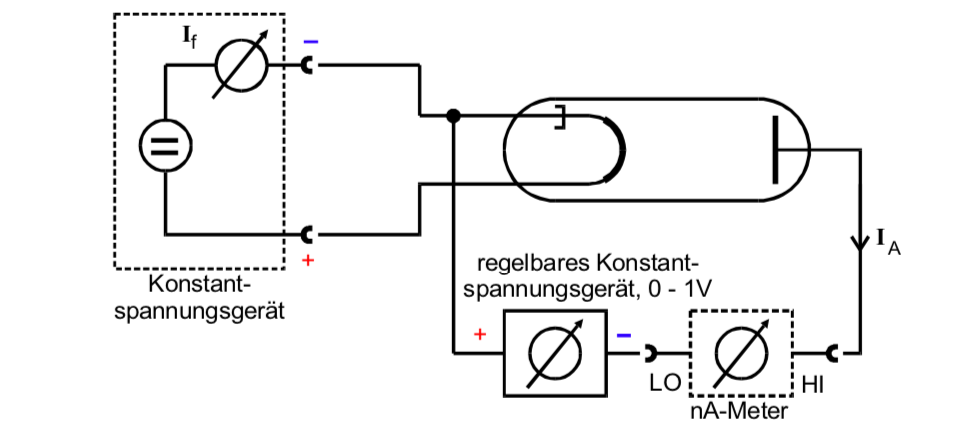
\includegraphics[width=0.8\textwidth]{content/8.png}
  \caption{Schaltung zur Aufnahme einer Anlaufstromkurve \cite{sample}}
  \label{fig:8}
\end{figure}
Da die auftretenden Ströme bei dem Anlauf im Nano-Bereich sind, muss ein entsprechend empfindliches Amperemeter verwendet werden.
Damit eine solche Genauigkeit erreicht werden kann, hat das Amperemeter einen Innenwiderstand von \SI{1}{\mega\ohm}. Dies verfälscht jedoch auch die Spannung,
weshalb bei der Auswertung auf die Korrektur der Spannung geachtet werden muss.
Die Messdaten werden in 0.1V Schritten aufgenommen, von 0V bis zu 1V.
Mit Hilfe dieser aufgenommenen Kennlinien wird die Auswertung vorgenommen.
